\section{Fundamentos de Mapas Web}
	
	\subsection{Coordenadas Geográficas}
	Coordenadas geográficas são usadas para expressar localizações no mundo. Existem vários sistemas de coordenadas diferentes. O sistema de coordenadas usado pelo Google Maps é o Word Geodetic System 84 (WGS84), que é o mesmo sistema que o Global Position System(GPS) usa.
	
	As coordenadas são expressas usando o conceito de latitude e longitude. Onde latitude mede do sul ao norte e longitude mede do oeste para o leste. No equador a latitude é 0. Isso significa que tudo abaixo do equador (hemisfério sul) possui uma latitude negativa, e tudo acima possui uma latitude positiva. Similarmente também existe uma linha zero para longitude. Ela é conhecida como meridiano, e por razões históricas passa por Greenwich, Inglaterra. Cada posição que é localizada a leste desta linha tem um número positivo e tudo a oeste tem um número negativo\cite[4]{livroGoogleApiV3}. 
	
	A \autoref{fig-coordenadas} permite uma melhor observação desses conceitos:
	\begin{figure}[htb]
	\caption{\label{fig-coordenadas} O centro do mundo na latitude 0 e longitude 0 reside em algum lugar a oeste da costa da África}
	\begin{center}
	    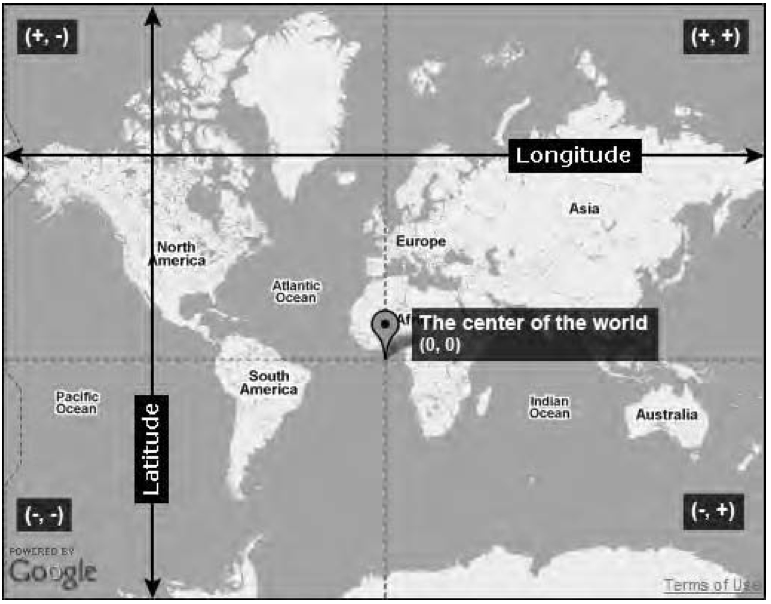
\includegraphics[scale=0.5]{goo-coordenadas}
	\end{center}
	\legend{Fonte: \cite[5]{livroGoogleApiV3}}
	\end{figure}
	
	Dessa forma é possível representar o mapa do mundo em uma imagem retangular que é projetada sobre o plano cartesiano.
	
	Caso seja necessário um maior grau de detalhamento, do mapa, basta que se aumente a resolução da imagem mantendo as proporções e relações entre as coordenadas (x,y), do plano cartesiano, com as coordenadas (longitude, latitude) que são usadas pelo mapa.
		
	\subsection{Zoom}
	As coordenadas de longitude e latitude servem para localizar um ponto numa imagem retangular, através de suas correspondentes x e y do plano cartesiano. Porém mapas também fornecem uma terceira coordenada conhecida como coordenada de Zoom.
	
	 Esta  coordenada controla qual o tamanho da imagem que será usada para projetar o mapa sobre o plano cartesiano. Usualmente, um mapa com coordenada zoom, ou nível de zoom, igual a zero possui uma imagem de tamanho 256x256 pixels. A cada incremento, da coordenada de zoom, dobra-se o tamanho da imagem usada para representar o mapa, e consequentemente o nível de detalhes. De forma que  para zoom=1 a imagem terá 512x512 pixels, para zoom=2 terá 1024x1024 e assim por diante. A \autoref{fig-zoomlevels} exemplifica esse processo:
	\begin{figure}[htb]
	\caption{\label{fig-zoomlevels} A cada incremento de zoom um mapa dobra a sua resolução de imagems}
	\begin{center}
	    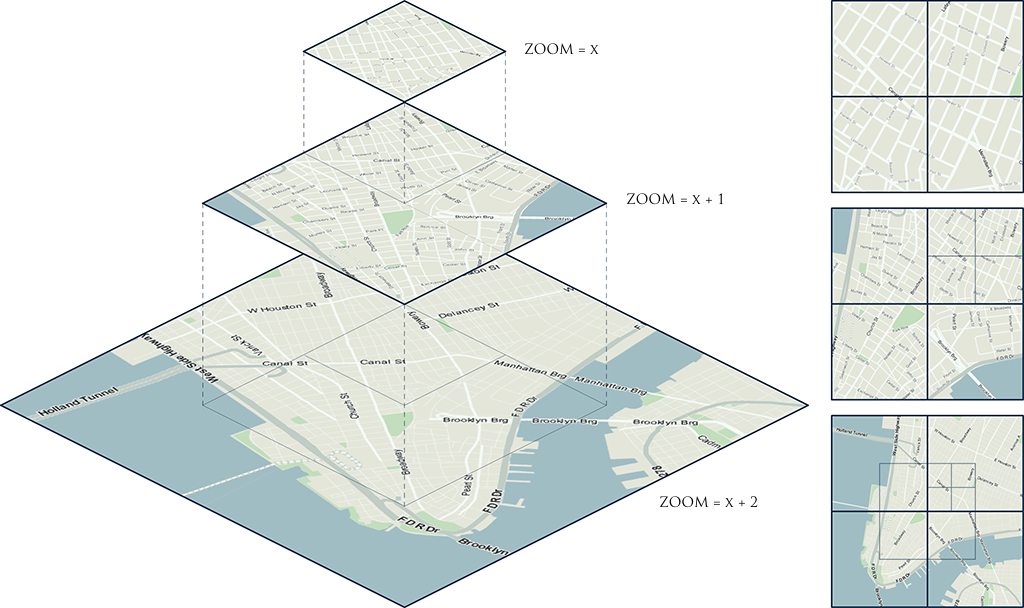
\includegraphics[scale=0.45]{tiles3d}
	\end{center}
	\legend{Fonte: http://workshops.opengeo.org/suiteintro/geowebcache/basics.html}
	\end{figure}

	Portanto para localizar uma posição  em um mapa web, de forma detalhada, precisamos de três coordenadas: latitude, longitude e zoom. Além disso, como o tamanho da imagem da projeção varia de acordo com o nível de zoom, o mapa precisa ajustar os valores das coordenadas latitude e longitude para que mantenham suas proporções para os diversos níveis de zoom.

\section{Estratégias para lidar com muitos marcadores\label{sec-estrategias}}
	Um problema comum, ao se trabalhar com mapas de crowdsourcing, é a enorme quantidade de marcadores necessários para representar os dados do mapa. Isto geralmente afeta a performance do mapa, pois quanto mais marcadores são inseridos mais lenta fica a exibição do mapa. 
	
	É difícil calcular exatamente o número máximo de marcadores que um mapa suporta antes de começar a ficar lento, pois a velocidade de exibição do mapa depende tanto do navegador quando do computador em que é exibido. Por exemplo, um mapa pode ser exibido bem rápido em um navegador como o Google Chrome e ao mesmo tempo ser lento quando exibido no Internet Explorer.\cite[177]{livroGoogleApiV3}
	
    Portanto, é necessário um estudo sobre as  estratégias para se lidar com o problema de exibição de muitos marcadores em um mapa. Em \cite[capítulo~9]{livroGoogleApiV3} o autor comenta sobre duas estratégias básicas para esse problema. A primeira, e mais óbvia, é reduzir o número de marcadores. A segunda estratégia consiste em agrupar os marcadores por algum grau de similaridades.
    
  \subsection{Reduzindo o número de marcadores}
  Existem muitos meios de se reduzir o número de marcadores, entre eles destacam-se as reduções via busca, filtro e otimização visual.
	\subsubsection{Busca}
	Para se reduzir  o número de marcadores exibidos no mapa pode-se fornecer um mecanismo de pesquisa ou busca no mapa. Dessa forma mesmo que o mapa possua milhões de marcadores, somente aqueles que satisfaçam os critérios da busca são exibidos.
	
	 \begin{figure}[htb]
	\caption{\label{fig-estrategiabusca}Busca como estratégia para redução do número de marcadores}
	\begin{center}
	    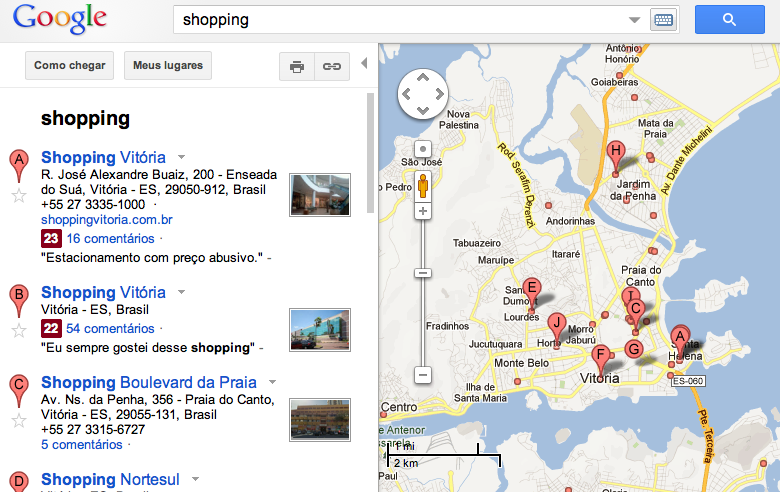
\includegraphics[scale=0.45]{estrategia-busca}
	\end{center}
	\legend{Fonte: http://maps.google.com}
	\end{figure}
	 
	 A \autoref{fig-estrategiabusca}  exemplifica isso ao mostrar o exemplo de busca no google maps. O google maps possui um catálogo enorme de informações, sobre diversas regiões geográficas. Mostrar todas essas informações ao mesmo tempo deixaria o mapa muito poluído, e praticamente inutilizável. Para que isso não aconteça é implementado o mecanismo de busca.
	
	 Na \autoref{fig-estrategiabusca} observa-se a exibição de uma busca pela palavra chave shopping. Nesta mesma região de interesse existem estabelecimentos de outras categorias como supermercados, lojas, padarias etc. Mas o google maps exibe apenas os marcadores relativos a categoria shopping, que é a palavra chave da busca. Ao fazer isso o mapa fica mais limpo e compreensivo.
	 
	
	\subsubsection{Filtro}
	De forma similar ao mecanismo de busca, um mapa também pode possuir um mecanismo para filtrar grupos de marcadores de acordo com algum critério de seleção do grupo. Dessa forma somente os marcadores que pertençam aos grupos marcados no filtro são exibidos no mapa. 
	
	Diferente do método de busca, este método permite ser mais específico e direto, pois cada campo do filtro é relacionado diretamente com alguma categoria contida nas informações. No método de busca esta relação é menos direta e depende do algorítimo de busca utilizado.  
	
	Como exemplo, ao utilizar-se do método de filtro para marcar duas categorias, obrigatoriamente, deve ser retornado o resultado para as duas categorias que foram marcadas. Já com o método de busca isto nem sempre é verdade, pois dependendo do algorítimo de busca ele pode entender que a busca por ``categoria 1 categoria 2'' é uma busca por duas categorias ou uma busca por uma categoria conhecida como ``categoria 1 categoria 2'', que obviamente não seria encontrada. 
		
	A \autoref{fig-estrategiafiltro} mostra um mapa com filtro a esquerda. Observa-se que apenas os marcadores dos grupos  ``Student Housing'' e ``Food/Dining''  são exibidos no mapa.
	 \begin{figure}[htb]
	\caption{\label{fig-estrategiafiltro}Filtro como estratégia para redução do número de marcadores}
	\begin{center}
	    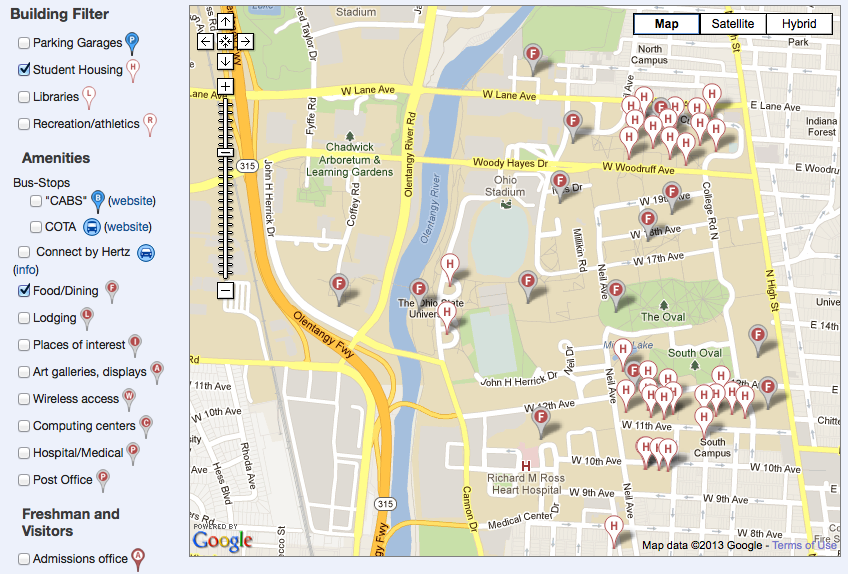
\includegraphics[scale=0.5]{estrategia-filtro}
	\end{center}
	\legend{Fonte: http://www.osu.edu/map/google.php}
	\end{figure}
	 
	\subsubsection{Otimização Visual}
	Nem sempre é preciso usar marcadores para representar dados de um mapa. Em alguns mapas faz mais sentido usar polígonos ou grupo de polígonos para representar um dado ao invés de simplesmente um ponto para o marcador. Por exemplo, ao exibir uma rota  não é necessário um marcador para cada vértice da rota, pois precisa-se apenas do desenho de uma linha, passando por cada vértice, para que a rota seja representada.
	
	A \autoref{fig-otimizacao} mostra um exemplo desse tipo de otimização. No mapa à esquerda, ela exibe uma rota com marcadores em cada vértice do trajeto percorrido. No mapa à direita, ela exibe a mesma rota só que sem colocar marcadores nos vértices do trajeto, deixando apenas um marcador para exibir o ponto de início do trajeto.
	
	 \begin{figure}[htb]
	\caption{\label{fig-otimizacao}Otimização Visual como estratégia para redução do número de marcadores}
	\begin{center}
	    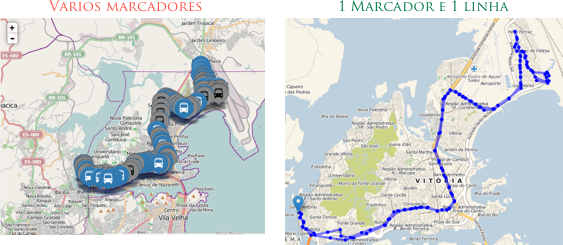
\includegraphics[scale=0.7]{estrategia-otimizacao}
	\end{center}
	\end{figure}
	
	Nesse exemplo, cada vértice da rota representa um ponto de parada para os ônibus que percorrem esse trajeto. Inicialmente, pode se achar necessário a exibição de marcadores nesses vértices como mecanismos de interação com os dados que eles representam. Por exemplo, os usuários do transporte público poderiam querer saber quais são os horários que determinados ônibus passam naquele ponto específico, e com um simples clique no marcador o mapa poderia exibir essa informação. 
	
	Porém, para que este tipo de interação seja possível o mapa teria que exibir os marcadores em cada vértice, que como mostrado na \autoref{fig-otimizacao} não é o melhor caminho. Felizmente, existe algumas alternativas para esse processo que não exigem a presença de um marcador. Por exemplo, ao clicar na linha da rota o mapa pode fazer uma busca, baseada em proximidade, e localizar o ponto que o usuário deseja saber mais informações. Após isso o mapa pode até exibir um marcador temporário como reforço visual do local que está sendo exibida a informação.
	

  \subsection{Agrupamento/Clustering\label{secagrupamento}}
  A segunda estratégia citada por \cite[capítulo~9]{livroGoogleApiV3} para reduzir o número de informações exibidas por um mapa, é conhecida como clustering, ou em português, agrupamento.
  
  A estratégia de agrupamento de marcadores consiste em agrupar marcadores que estejam próximos, por algum critério de proximidade, e exibir apenas um marcador para cada grupo e um marcador para cada marcador individual, que não pertença a nenhum grupo. Ou seja, em vez de exibir um marcador individual para cada marcador são exibidos marcadores para grupos e marcadores individuais. 
  
  Nessa estratégia os grupos variam de acordo com o zoom. Ou seja, ao fazer zoom em grupo, o grupo se divide em subgrupos menores e, se for o caso, em marcadores individuais.
  
   O processo contrário também ocorre ao diminuirmos o zoom de um grupo. Neste caso o grupo pode se agrupar com grupos vizinhos e formar um novo grupo como mais elementos, de forma, que em alguns mapas, no zoom=0 o mapa exibe apenas um marcador representando o grupo com todos os marcadores do mapa.

   Existem diversos métodos para agrupamento de marcadores, mas os mais comuns são implementados usando algum dos seguintes parâmetros para agrupamento: agrupamento por grade, por distância, ou por região.
     
		\subsubsection{Agrupamento Por Grade}
		Agrupamento baseado em grade é provavelmente a abordagem mais comum para agrupar marcadores. Esta abordagem, divide o mapa em uma grade e agrupa todos os marcadores de cada quadrado em um grupo. 
		
		Apesar de ser uma técnica eficiente, ela possui limitações óbvias, pois pode levar a resultados indesejados. Por exemplo, considere dois marcadores próximos mas localizados em quadrados diferentes da grade. Neste caso, eles não serão agrupados no mesmo grupo. Para exemplificar isso, veja a \autoref{fig-porgrelha}. 

\begin{figure}[htb]
	\caption{\label{fig-porgrelha}Estes dois marcadores não serão agrupados pois residem em quadrados diferentes da grade}
	\begin{center}
	    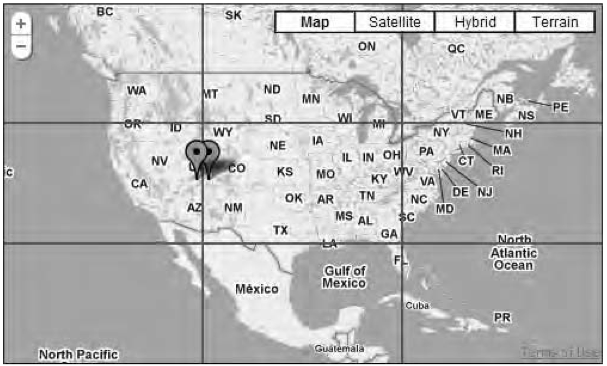
\includegraphics[scale=0.7]{porgrelha}
	\end{center}
		\legend{Fonte: \cite[figura 9.6]{livroGoogleApiV3}}
\end{figure}

		\subsubsection{Agrupamento Por Distância}
			Nesta técnica, não ocorre o problema comentado no agrupamento por grade, pois nela é observado cada marcador e para cada um é procurado marcadores vizinhos, se os marcadores forem próximos o suficiente eles são colocados no mesmo grupo.
		
			Alguns podem achar esta técnica problemática para certos mapas. Pois por agrupar marcadores próximos entre si, os grupos não possuem uma localização fixa como acontece no agrupamento por grade. Assim no agrupamento por distancia os grupos podem aparecer em posições aleatórias que podem não fazer sentido para o usuário que observa o mapa.
	
		\subsubsection{Agrupamento Por Região}
			No agrupamento por região, define-se diferentes regiões geográficas como países, estados, cidades. E todos os marcadores, de cada região, podem ser agrupados em um grupo para representar a região. Além disso, também é possível definir em que nível de zoom os grupos serão quebrados em subgrupos. 
			
			A vantagem é que fica fácil criar grupos que fazem mais sentido para o usuário. Pois, um agrupamento que siga a ordem Pais > Estado > Cidade é mais natural para o usuário do que um que considere apenas a proximidade.
			
			A desvantagem dessa técnica é o esforço para implementá-la  \cite[182]{livroGoogleApiV3} já que a definição dos grupos não pode ser facilmente automatizada. Essa dificuldade ocorre devido a natureza de como é organizado a hierarquia das regiões, que varia de país para país, sendo necessário em alguns casos o uso de tabelas para conversão\footnote{Até a definição do que é uma autoestrada precisa de uma tabela de conversão entre paises: \url{http://wiki.openstreetmap.org/wiki/Highway:International_equivalence}}.
			
		\subsubsection{Estilos de visualização de agrupamento}
		A representação mais simples de um agrupamento pode ser feita por meio de um marcador. Porém, o marcador por si só não expressa muita informação. Não é possível saber a dimensão do grupo ou a natureza de seus elementos observando apenas um marcador.
		
		Uma alternativa é usar marcadores com tamanhos diferentes de acordo com o tamanho do grupo. Mas, neste caso,tem-se o problema de ter que classificar um tamanho padrão para determinados marcadores. Pode-se, também, usar cores para representar a dimensão do grupo, onde grupos menores tenderiam para o verde e grupos maiores para o vermelho.
		
		Uma solução bastante comum é uma mistura das soluções anteriores. Onde usa-se um marcador com tamanho diferente de acordo com o número de elementos e cores para maximizar a percepção. Além disso, acrescenta-se uma legenda exibindo o número total de elementos do grupo. Veja a \autoref{fig-visual-agrupamento}
		
		
\begin{figure}[htb]
	\caption{\label{fig-visual-agrupamento}Usando tamanho e cor do marcador para representar a dimensão do grupo}
	\begin{center}
	    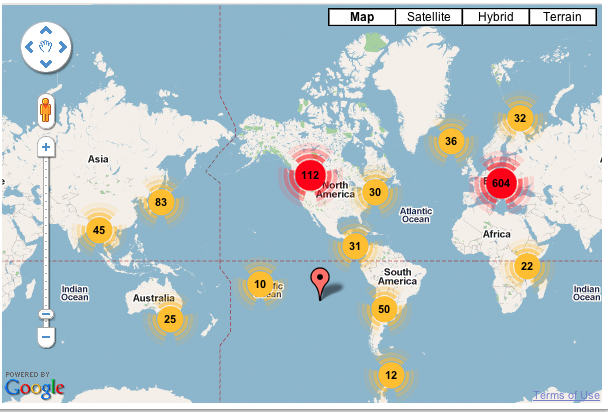
\includegraphics[scale=0.5]{visual-agrupamento}
	\end{center}
		\legend{Fonte: \url{https://developers.google.com/maps/articles/toomanymarkers}}
\end{figure}

	Alguns mapas, possuem dados que permitem uma visualização mais complexa. Para esses tipos de mapa é possível substituir o marcador por uma imagem, gráfico ou forma que represente o grupo.  Por exemplo, uma mapa que mostre as compras de todos os clientes de uma rede de supermercados poderia agrupar os dados inicialmente por loja e na visualização exibir um gráfico de vendas para representar cada grupo. Veja a \autoref{fig-mapa-graficos}.
	
\begin{figure}[htb]
	\caption{\label{fig-mapa-graficos}Usando gráficos para representar agrupamentos}
	\begin{center}
	    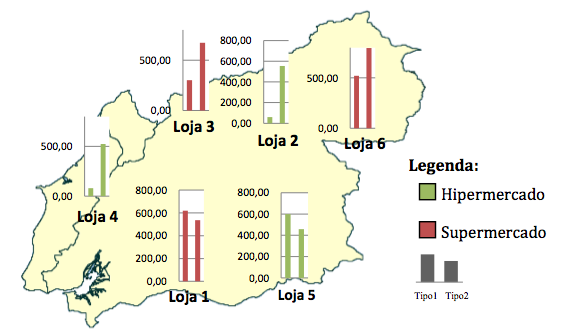
\includegraphics[scale=0.5]{mapa-graficos}
	\end{center}
		\legend{Fonte: \cite[figura 65]{silva2010solap+}  }
\end{figure}

	Além disso, os gerentes dessas lojas,  poderiam efetuar um zoom no gráfico da loja que gerenciam e ver os subgrupos divididos por bairros, com cada grupo exibindo o gráfico de vendas do bairro, permitindo aos gerentes a criação de uma estratégia de marketing localizada.
	
\section{Algorítimos de agrupamento}	
	Basicamente os algorítimos de agrupamentos de pontos podem ser classificados em quatro categorias: (i) método por partição (ii) método hierárquico (iii) método baseado em densidade (iv) método baseado em grade. Isto é ilustrado na \autoref{fig-algoritimos} onde SILVA destaca os potenciais melhores algorítimos para este tipo de problema. Com exceção dos algorítimos k-Means e k-Medoid que foram introduzidos apenas por motivos históricos \cite[35]{silva2010solap+}.
	
	Observa-se que em \cite[capítulo 2]{silva2010solap+} é feito um estudo mais aprofundado sobre os principais algorítimos de agrupamentos de pontos. Por isso, nesta seção será descrito apenas o algorítimo que engloba o contexto deste trabalho. Ou seja, o algorítimo WaveCluster que é baseado no método de grade. 
		
\begin{figure}[htb]
	\caption{\label{fig-algoritimos}Principais algorítimos de agrupamentos de pontos}
	\begin{center}
	    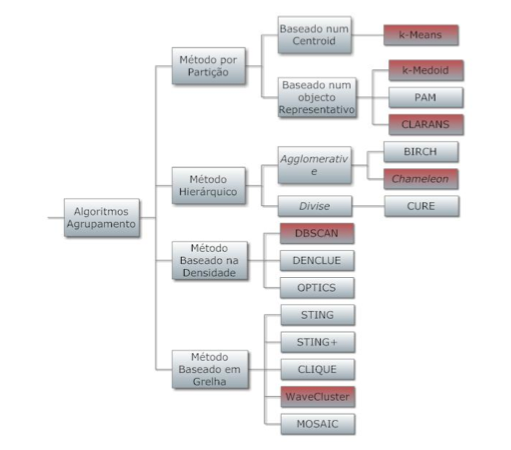
\includegraphics[scale=0.8]{algoritimos}
	\end{center}
		\legend{Fonte: \cite[figura 15]{silva2010solap+}  }
\end{figure}

		\subsection{Métodos baseados em grade}
		Como já foi comentado na \autoref{secagrupamento}, agrupamentos baseados em grade são aqueles que dividem o espaço do mapa em uma grade e agrupa os marcadores de cada quadrado ou célula da grade.  Ou seja, algorítimos baseados em grade são aqueles que usam o agrupamento por grade como parâmetro de agrupamento. 
		Pode se observar na \autoref{fig-algoritimos} que os principais algorítimos são: STING, STING+, CLIQUE, WaveCluster e MOSAIC. E, apesar de não ser o mais indicado para o contexto SOLAP+ que SILVA estudava, o melhor entre os algorítimos baseados em grade é o WaveCluster.
		
		
		\subsubsection{WaveCluster}
			Uma boa abordagem para agrupamentos deve ser eficiente e detectar grupos de formas arbitrárias. Ela também tem que ser insensível a dados discrepantes e a ordem de entrada dos dados.
			
			O algorítimo WaveCluster atende todos esses requisitos. Sua definição completa é encontrada em \cite{wavecluster} mas em resumo o algorítimo faz o seguinte:
\begin{algorithm}
\caption{WaveCluster}
\textbf{Entrada} Vetores de características dos objetos de dados multidimensionais

\textbf{Saida} Objetos agrupados
\begin{enumerate}
\item Quantizar o espaço de características, atribuir objetos as celulas da grade.
\item Aplicar a transformação $wavelet^1$ no espaço de características quantizado.
\item Encontrar os componentes conectados (clusters) nas sub-bandas
\item Transformar o espaço original, em diferentes níveis.
\item Atribuir rótulos as células.
\item Criar a tabela de pesquisa.
\item Mapear objetos aos clusters/grupos.
\end{enumerate}
\end{algorithm}
\footnotetext{Uma transformada de wavelet é uma tecnica de processamento de sinais que decompõe o sinal em diferentes sub-bandas de frequencia.} 

O WaveCluster possui complexidade O(n). Além disso, por causa do uso das técnicas de processamento de sinais a propriedade de multi-resolução, ou agrupamento nos níveis hierárquicos, também é aplicada ao WaveCluster.

O seu uso não é limitado apenas à dados espaciais, o algorítimo WaveCluster pode ser aplicado a qualquer conjunto de atributos com valores numéricos ordenados.
	
%
%
%\section{Planilhas eletrônicas e Mapas}
%\subsection{Domínios de conhecimento}
%Mostra a importância do uso de planilhas \cite{credinePlanilha} 
%\subsection{O desafio chinês}
%mostra o uso de planilhas pelo governo chines e as dificuldades encontradas \cite{chinaPlanilha}
%
%\subsection{Usando planilhas como fonte de dados para Mapas Geográficos}
%Mostra \cite{lieberman2009spatio}